\chapter{Marco Teórico} \label{ch:m_teorico}

% estructura
\section{Sistemas de Conducción Autónoma}
-
    \subsection{Niveles de Autonomía}

    \subsection{Arquitectura de un sistema de conducción autónoma}
    % \subsection{Aprendizaje Profundo}


\section{Visión por computador}
-
    \subsection{Procesamiento de imágenes}
    \subsection{Filtrado}

\section{Redes Neuronales Artificiales}
-
    \subsection{Aprendizaje Automático}

    El aprendizaje automático surge de la necesidad de poder encontrar una representación útil
    de las ingentes cantidades de datos que se generan 
        \subsubsection{Aprendizaje supervisado}
        Dentro del campo del aprendizaje au
        \subsubsection{Aprendizaje no supervisado}
        \subsubsection{Aprendizaje por refuerzo}
    
    \subsection{Aprendizaje Profundo}
        \subsubsection{Redes neuronales profundas}
        \subsubsection{Funciones de activación}
        \subsubsection{Funcion de costo}
        \subsubsection{Gradientes y retropropagación}
        \subsubsection{Diseño de Arquitecturas}

    \subsection{Redes Neuronales Convolucionales}
    Las redes neuronales convolucionales son un tipo especializado de red neuronal que 
    sirven para procesar datos de tipo "grilla" \cite{Goodfellow-et-al-2016}. Algunos ejemplos 
    de datos de tipo grilla que se pueden mencionar son los siguientes:
    \begin{itemize}
        \item \textbf{Series de tiempo.} Grilla de una dimensión tomados en intervalos regulares de tiempo.
        \item \textbf{Imágenes digitales.} Grilla de pixeles de dos o más dimensiones (Escala de grises, RGB).
    \end{itemize}

    Las también llamadas redes convolucionales, han demostrado un éxito impresionante en diversas 
    aplicaciones prácticas especialmente en el campo de la visión por computador y el procesamiento de texto y lenguaje natural. 
    El término ``red neuronal convolucional'' proviene del hecho de que en este tipo 
    de redes neuronales se utiliza una operación matemática llamada \textbf{convolución}, siendo la convolución 
    una operación lineal especializada para procesar datos de tipo grilla.

    En los párrafos posteriores, se procede a describir la operación de convolución en el contexto de 
    redes neuronales, pues, no siempre la definición de la misma corresponde con el concepto de convolución
    usado en distintos campos de la ciencia y la ingeniería.

        \subsection{Operación de convolución}
        En su forma más general, la convolución es una operación entre dos funciones reales y su definición se puede introducir
        usando el concepto de un promedio ponderado. Sea una función $x(t)$ dependiente del tiempo, 
        tanto $x$ como $t$ son números reales; en este caso, la función $x$ puede entenderse como una serie de medidas
        en un instante de tiempo $t$. Considérese una segunda función de ponderación $w(\tau)$ donde $\tau$ es la antiguedad 
        de una medida. Si se aplica la función de ponderación en cada instante de tiempo, se puede obtener una nueva función 
        definida por:
        \begin{equation}
            s(t) = \int x(\tau)w(t - \tau) d\tau
        \end{equation} 
        Esta operación es llamada la \textit{operación de convolución} y es denotada tradicionalmente con un asterisco:
        \begin{equation}
            s(t) = (x\ast w)(t)
        \end{equation}
        En el ejemplo de la ponderación, $w$ debe ser una función de densidad de probabilidad válida, o la salida no podrá
        ser considerada como un promedio ponderado. Además, $w$ también debe ser $0$ para cualquier $t<0$, esta última 
        característica se denomina comunmente como el principio de ``causalidad''. En general, la convolución está 
        definida para cualquier función en la cual la integral anteriormente declarada esté definida y puede ser 
        usada para otros propósitos aparte de promedios ponderados.

        Hablando en términos de una red neuronal convolucional, el primer argumento (en el ejemplo, la función $x$) 
        es comunmente referido como la \textbf{entrada}, y el segundo argumento ($w$, en el ejemplo) es referido 
        como el \textbf{kernel}. La salida, a su vez, es normalmente referida como el \textbf{mapa de características}.
        
        Por su parte, cuando se trata de señales digitales, como los datos en una computadora, el tiempo tiene una 
        naturaleza discreta, es decir, que los datos estarán disponibles en intervalos regulares de tiempo. En este 
        caso, el índice de tiempo $t$ puede tomar solamente valores enteros y, entonces, es válido asumir 
        que tanto $x$ como $w$ estan definidos solamente para valores enteros de $t$. De este modo, 
        se puede definir la convolución discreta:
        \begin{equation}
            s(t) = (x \ast w)(t) = \sum_{\tau=-\infty}^{\infty}x(\tau)w(t-\tau)
        \end{equation}

        En el contexto de las aplicaciones de aprendizaje automático o, más específicamente, aprendizaje profundo,
        la entrada es usualmente un arreglo multidimensional de datos, y el kernel es usualmente un arreglo 
        multidimensional de parámetros que se adaptan en el proceso de aprendizaje. 

        \subsubsection{Procesamiento de imágenes con redes neuronales convolucionales}

        % TODO: poner un grafico de la convolucion en 2d de una imagen 

        La operación de convolución se usa frecuentemente sobre datos con más de una dimensión. Las imágenes digitales 
        son un perfecto ejemplo de un arreglo multidimensional de datos. Una imagen digital se representa mediante una
        matriz con filas y columnas, donde cada elemento se denomina pixel y contiene información acerca de la intensidad
        o luminancia, para una imagen en escala de grises o el nivel de color para distintos canales en una imagen a color.
        Si se toma el ejemplo de la imagen en escala de grises, se tiene una entrada o imagen bidimensional $I$ con un
        kernel bidimensional correspondiente $K$:

        \begin{equation} \label{eq:conv2d}
            S(i,j)=(I\ast K)(i,j) = \sum_{m} \sum_{n} I(m,n)K(i-m,j-n)
        \end{equation}

        Dado que la convolución es conmutativa, se puede reescribir la ecuación \ref{eq:conv2d} como:

        \begin{equation}
            S(i,j)=(K\ast I)(i,j) = \sum_{m} \sum_{n} I(i-m,j-n)K(m,n)
        \end{equation}

        Frecuentemente, la última fórmula es la más utilizada en librerías de aprendizaje profundo 
        por su sencillez en la implementación en un sistema computacional, esto, dado que existe menos 
        variación en el rango de valores válidos de $m$ y $n$.

        \subsubsection{Aprendizaje de representaciones internas}
        Una de las preguntas clave en la visión por computador es el cómo generar una buena y significativa
        representación interna de una imagen, dado que la mayor parte de la imagen corresponde con pixeles que no 
        aportan mucha información relevante a la tarea asignada. Por ejemplo, si se quisiera detectar 
        un rostro dentro de una imagen, normalmente se suele encontrar una representación que ayude a aislar solamente 
        las porciones de la imagen que pueden contener el rostro, tales como la búsqueda de contornos, bordes y 
        características típicas de un rostro. Antes de la aparición de las redes convolucionales, estas representaciones 
        se hallaban de manera manual y gracias al conocimiento de expertos en el área del procesamiento de imágenes. 
        La definición de características y mapas de características era comunmente conocida como la 
        \textit{ingeniería de características}, en la cual los expertos creaban descriptores para tareas específicas con 
        una gran inversión de tiempo en la sintonización fina de los mismos. 

        % TODO: poner el ejemplo de viola jones 

        En contraste con el anterior enfoque, las redes convolucionales generan sus propias representaciones internas
        de manera automática gracias al aprendizaje de los parámetros de cada uno de los kernels que componen las distintas 
        capas de la red neuronal. En principio, las redes convolucionales se inspiraron en el trabajo de Hubel y Wiesel 
        sobre la corteza visual primaria de un gato\cite{lecun2010convolutional}. En dicho trabajo, se logró identificar células simples que respondían
        de manera sobresaliente a distintas orientaciones con campos receptivos locales. Éstas células receptivas simples 
        se pueden corresponder con los kernels de convolución usados en las redes convolucionales por la sencillez y la 
        localidad de su campo de receptividad.

        Posteriormente, las redes convolucionales ganaron una gran popularidad debido a su rendimiento en tareas de 
        clasificación de imágenes y detección y reconocimiento de objetos en imágenes. El primer hito de su capacidad 
        para procesar imágenes de manera efectiva fue en concurso de clasificación de imágenes de ImageNet, donde 
        el equipo de Geoffrey Hinton logró sobrepasar el mejor resultado en precisión de clasificación por un gran márgen 
        usando una arquitectura de red convolucional \cite{krizhevsky2012imagenet}. En este trabajo, se pudo apreciar con 
        gran detalle las ventajas del enfoque del aprendizaje de representaciones internas en una red convolucional.

        \begin{figure}[!h] 
            \centering
            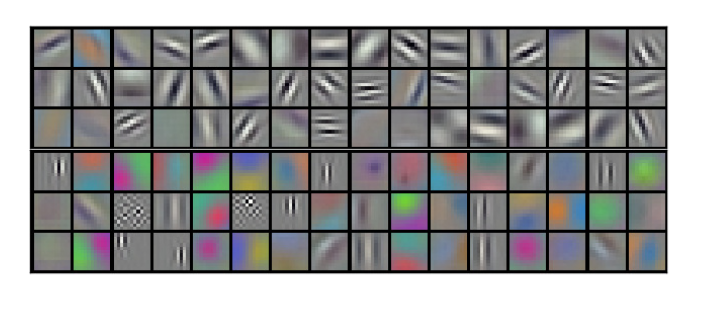
\includegraphics[width=0.75\textwidth]{img/fmap_imagenet}
            \caption{Kernels convolucionales de tamaño $11 \times 11 \times 3$ en la primera capa convolucional. Fuente: \cite{krizhevsky2012imagenet} }
            \label{fig:fmap_imagenet}
        \end{figure}
            
        Tal como se puede apreciar en la Figura(\ref{fig:fmap_imagenet}), en la primera capa convolucional, 
        los kernels de convolución corresponden con representaciones básicas en una imagen como la búsqueda de 
        bordes en distintas orientaciones, esto va acorde a lo establecido anteriormente en el modelo de 
        la corteza visual de un gato. Puede decirse entonces que las redes convolucionales emulan, en cierto modo, 
        al proceso biológico de visión en animales.

    \subsection{Sistemas de Aprendizaje Fin a Fin}

\section{Modelo cinemático del vehículo}
-
    \subsection{Ecuaciones de movimiento}


